		\documentclass[10pt,a4paper]{article}
\usepackage[utf8]{inputenc}
%\usepackage[french]{babel}
\usepackage{tikz-network}
\usepackage{tikz}
\usepackage{graphics,multirow}
\usepackage{subcaption}
\usepackage{array}
\usepackage{xcolor}
\PassOptionsToPackage{hyphens}{url}
\usepackage{hyperref}
\usepackage{amsmath}
\usepackage{amsfonts}
\usepackage{amssymb}
\usepackage{mathtools}
\usepackage[backend=biber,style=numeric,sorting=ynt]{biblatex}
\addbibresource{report.bib}
 \hypersetup{
 %   bookmarks=true,         % show bookmarks bar?
 %   unicode=false,          % non-Latin characters in Acrobat’s bookmarks
 %   pdftoolbar=true,        % show Acrobat’s toolbar?
 %   pdfmenubar=true,        % show Acrobat’s menu?
 %   pdffitwindow=false,     % window fit to page when opened
 %   pdfstartview={FitH},    % fits the width of the page to the window
 %   pdftitle={My title},    % title
 %   pdfauthor={Author},     % author
 %   pdfsubject={Subject},   % subject of the document
 %   pdfcreator={Creator},   % creator of the document
 %   pdfproducer={Producer}, % producer of the document
 %   pdfkeywords={keyword1, key2, key3}, % list of keywords
 %   pdfnewwindow=true,      % links in new PDF window
    colorlinks=true,       % false: boxed links; true: colored links
    linkcolor=blue,          % color of internal links (change box color with linkbordercolor)
    citecolor=blue,        % color of links to bibliography
    filecolor=blue,         % color of file links
    urlcolor=blue        % color of external links
}
%% COLORS %%
%
\definecolor{mygreen}{RGB}{0,214,0}
%% MACROS %%

\newcommand\von{{\textsc{Von}}}
\newcommand\fon{{\textsc{Fon}}}
\newcommand\hon{{\textsc{Hon}}}
\newcommand\fston{$1^{\mathrm{st}}${\textsc{on}}}
\newcommand\nrep{N_{\mathrm{rep}}}
\newcommand\uprvec{\Pi_{\mathrm{Von}}^{\mathrm{U}}}
\newcommand\bprvec{\Pi_{\mathrm{1}}^{\mathrm{B}}}
\newcommand\hprvec{\Pi_{\mathrm{Von}}}
\newcommand\fprvec{\Pi_{\mathrm{1}}}
\newcommand\urank{K_{\mathrm{Von}}^{\mathrm{U}}}
\newcommand\brank{K_{\mathrm{1}}^{\mathrm{B}}}
\newcommand\hrank{K_{\mathrm{Von}}}
\newcommand\frank{K_{\mathrm{1}}}
\newcommand\vrank{K_{\mathrm{V}}}
\newcommand\reprank{K_{\mathrm{rep}}}
\newcommand{\red}[1]{\textcolor{red}{#1}}
\newcommand{\tbd}[1]{\textcolor{blue}{{\textbf{To do: #1}}}}
\newcommand{\ask}[1]{\textcolor{red}{{\textbf{Question: #1}}}}
\newcommand\mems{\textit{memory nodes}}
\newcommand\kin{k_{\mathrm{in}}}
\newcommand\kout{k_{\mathrm{out}}}
\newcommand\uhonpr{Unbiased HON PR}
\newcommand\honpr{HON PR}
\newcommand\pr{1stON PR}
\newcommand\bpr{1stON Biased PR}
%\author{Célestin Coquidé}
\title{Analysis of the Pearson Correlation Network Between Methylated DNA and RNA in the Context of Breast Cancer Tissues}
\date{\today}
\begin{document}
\maketitle
\section{Methods and Data}
We used an open access cancer dataset from GDC Data Portal. From raw data consisting in methylated DNA and RNA's beta-values for up to 841 tumorous and normal breast tissues, we built a Matrix of Pearson Correlation Coefficients between Methylated DNA and RNA from these beta-values. A network representing the Pearson correlation coefficients between pairs (M-DNA,RNA) consists in a bipartite graph with coefficients as weight of the links. Two possibilities are considered either the correlation is positive or negative. Therefore we consider a signed bipartite graph with undirected links.
\subsection{Construction of the Signed Bipartite Network}
A negative correlation coefficient between two random variables $A$ and $B$, $\rho(A,B)<0$, means that the more $A$ is observed, the lower $B$ is observed, whereas a positive value $\rho(A,B)>0$ tells that the more $A$ is present the more is $B$. By constructing the projected network (DNA-M projection and RNA projection), we can infer indirect positive and negative correlations between the molecules. Therefore by assigning sign to the links of the correlation network, we can easily infer the complementary correlation. Let $A$ and $C$ be two DNA-M sites and $B$ be a RNA molecule. If $\rho(A,C)$ and $\rho(B,C)$ are two measured Pearson correlation coefficients and have associated links $A-C$ and $B-C$ in the signed bipartite network, the DNA-M projection network will contain the signed link $A-B$ representing the complementary correlation coefficient $\rho(A,B)$. The complementary rules are the following: The complementary correlation is positive (negative) if both correlations have the same sign (different signs). However, correlations are not necessarily transitive meaning that for some $\rho(A,C)$ and $\rho(B,C)$ with absolute value big enough ($\approx 0.6$ for instance), the complementary correlation $\rho(A,B)$ might represent a very low correlation \cite{langford12}. The transitivity occurs when both correlations are large enough such that
\begin{equation}
\rho(A,C)^{2} + \rho(B,C)^{2} > 1.
\label{eq:transitivy}
\end{equation}

In order to respect the criteria defined in eq.~\ref{eq:transitivy}, we keep the Pearson correlation coefficient matrix elements $B_{ij}$ being greater than $\frac{1}{\sqrt{2}}$.

\paragraph{Projections}
The bipartite adjacency matrix $B$'s column index refers to the RNAs and its row to the DNA-Ms. Is elements are complex numbers $z=a+ib$ such that for a pair $i,j$, $Re(B_{ij})=1$ and $Im(B_{ij})=0$ if $\rho(i,j)>0$ or $Re(B_{ij})=0$ and $Im(B_{ij})=1$ otherwise. For a real bipartite adjacency matrix, the projection adjacency matrices are $A_{r}=(BB^{T})_{nd}$ and $A_{c}=(B^{T}B)_{nd}$ for row and column projections respectively, where $(X)_{nd}$ denotes the matrix $X$ with diagonal elements set to zero. In this case the value $A_{ij}$ is the number of common neighbor $k$, $i$ and $j$ shares in the bipartite network. In a similar way we compute the signed-row-projection adjacency matrix $A_{r}$ as following
\begin{equation}
A_{r}=[Re(BB^{\dagger}) + i.Im(BB^{T})]_{nd}
\label{eq:signedproj}
\end{equation}
where $X^{\dagger}$ denoted the transpose conjugate of the complex matrix $X$. Finally the signed-column-projection adjacency matrix $A_{c}$ is computed by replacing $B$ with $B^{T}$. The number of neighbor $k$ that $i$ and $j$ share a correlation of same sign is $Re(A_{r}(i,j))$, these are positive complementary correlations. Similarly $Im(A_{r}(i,j))$ is the number of negative complementary correlations between DNA-M sites $i$ and $j$.

Here after is an example of a signed bipartite network (see Fig.~\ref{fig:ex_a}) composed of three methylated DNA $m_{1}$, $m_{2}$, and $m_{3}$ and four RNA $r_{1}$, $r_{2}$, $r_{3}$ and $r_{4}$. The complex bipartite adjacency matrix and its conjugate transposed are
\begin{equation}
B=\begin{pmatrix}
1&i&0&1\\
i&i&0&0\\
0&i&1&1
\end{pmatrix}
B^{\dagger}=\begin{pmatrix}
1&-i&0\\
-i&-i&-i\\
0&0&1\\
1&0&1
\end{pmatrix}
\label{eq:example}
\end{equation}
This lead to the projected networks (Fig.~\ref{fig:ex_b} and \ref{fig:ex_c}) represented by the matrices
\begin{equation}
A_{r}=\begin{pmatrix}
0&1+i&2\\
1+i&0&1\\
2&1&0
\end{pmatrix}
A_{c}=\begin{pmatrix}
0&1+1&0&1\\
1+i&0&i&2i\\
0&i&0&1\\
1&2i&1&0
\end{pmatrix}
\label{eq:example2}
\end{equation}
\begin{figure}[h]
\resizebox{\textwidth}{!}{%
%\centering
\begin{subfigure}{0.6\textwidth}
\centering
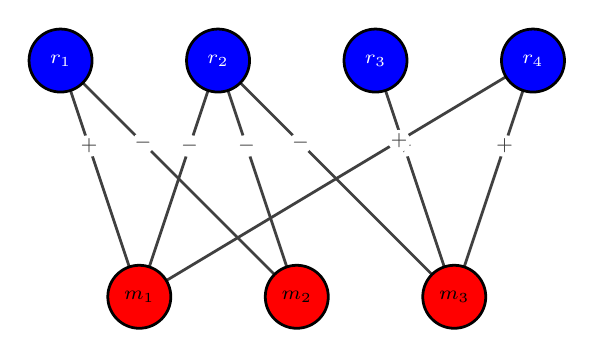
\begin{tikzpicture}
%\Text[x=0,y=3]{\textbf{HON}}
\Vertex[color=red,x=-2,y=-2,label={$m_{1}$},size=0.8,fontscale=1]{r1}
\Vertex[color=red,x=0,y=-2,label={$m_{2}$},size=0.8,fontscale=1]{r2}
\Vertex[color=red,x=2,y=-2,label={$m_{3}$},size=0.8,fontscale=1]{r3}
\Vertex[color=blue,x=-3,y=1,fontcolor=white,label={$r_{1}$},size=0.8,fontscale=1]{c1}
\Vertex[color=blue,x=-1,y=1,fontcolor=white,label={$r_{2}$},size=0.8,fontscale=1]{c2}
\Vertex[color=blue,x=1,y=1,fontcolor=white,label={$r_{3}$},size=0.8,fontscale=1]{c3}
\Vertex[color=blue,x=3,y=1,fontcolor=white,label={$r_{4}$},size=0.8,fontscale=1]{c4}
\Edge[label=$+$,distance=0.7,lw=1pt](r1)(c1)
\Edge[label=$-$,distance=0.7,lw=1pt](r1)(c2)
\Edge[label=$-$,distance=0.7,lw=1pt](r2)(c1)
\Edge[label=$-$,distance=0.7,lw=1pt](r2)(c2)
\Edge[label=$-$,distance=0.7,lw=1pt](r3)(c2)
\Edge[label=$+$,distance=0.7,lw=1pt](r3)(c3)
\Edge[label=$+$,distance=0.7,lw=1pt](r1)(c4)
\Edge[label=$+$,distance=0.7,lw=1pt](r3)(c4)
%\Edge[Direct,lw=2pt,bend=15](1)(1C)
\end{tikzpicture}
\caption{Signed bipartite network}
\label{fig:ex_a}
\end{subfigure}
\newline
\begin{subfigure}{0.3\textwidth}
\centering
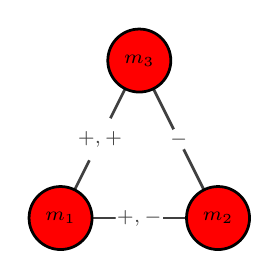
\begin{tikzpicture}
%\Text[x=0,y=3]{\textbf{HON}}
\Vertex[color=red,x=-2.5,y=-0.5,label={$m_{1}$},size=0.8,fontscale=1]{r1}
\Vertex[color=red,x=-0.5,y=-0.5,label={$m_{2}$},size=0.8,fontscale=1]{r2}
\Vertex[color=red,x=-1.5,y=1.5,label={$m_{3}$},size=0.8,fontscale=1]{r3}
\Edge[label=${+,-}$,distance=0.5,lw=1pt](r1)(r2)
\Edge[label=${+,+}$,distance=0.5,lw=1pt](r1)(r3)
\Edge[label=$-$,distance=0.5,lw=1pt](r2)(r3)
\end{tikzpicture}
%\vspace{20pt}
\caption{}Projection onto the methylated DNAs
\label{fig:ex_b}
\end{subfigure}
\begin{subfigure}{0.3\textwidth}
\centering
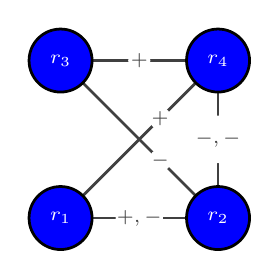
\begin{tikzpicture}
\Vertex[color=blue,x=0.5,y=-0.5,fontcolor=white,label={$r_{1}$},size=0.8,fontscale=1]{c1}
\Vertex[color=blue,x=2.5,y=-0.5,fontcolor=white,label={$r_{2}$},size=0.8,fontscale=1]{c2}
\Vertex[color=blue,x=0.5,y=1.5,fontcolor=white,label={$r_{3}$},size=0.8,fontscale=1]{c3}
\Vertex[color=blue,x=2.5,y=1.5,fontcolor=white,label={$r_{4}$},size=0.8,fontscale=1]{c4}
\Edge[label=${+,-}$,distance=0.5,lw=1pt](c1)(c2)
\Edge[label=$+$,distance=0.7,lw=1pt](c1)(c4)
\Edge[label=$-$,distance=0.3,lw=1pt](c2)(c3)
\Edge[label=${-,-}$,distance=0.5,lw=1pt](c2)(c4)
\Edge[label=$+$,distance=0.5,lw=1pt](c3)(c4)
\end{tikzpicture}
%\vspace{20pt}
\caption{Projection onto the RNAs}
\label{fig:ex_c}
\end{subfigure}
}
\caption{Exemple of signed bipartite network and its projections.}
\label{fig:toynet}
\end{figure}
\section{Preliminary Results}

\subsection{Projected networks statistics}
With the use of a threshold satisfying eq.\ref{eq:transitivy}, we have $683$ RNAs and $4687$ M-DNAs present in both projections. About $30\%$ ($90\%$) of the RNAs (M-DNAs) are involved in both negative and positive complementary correlations. Hereafter is presented statistics and preliminary figures for the projected networks' connected components (CC). We considered the only positive, only negative and both positive and negative signed projections.
\begin{figure}[h!]
\centering
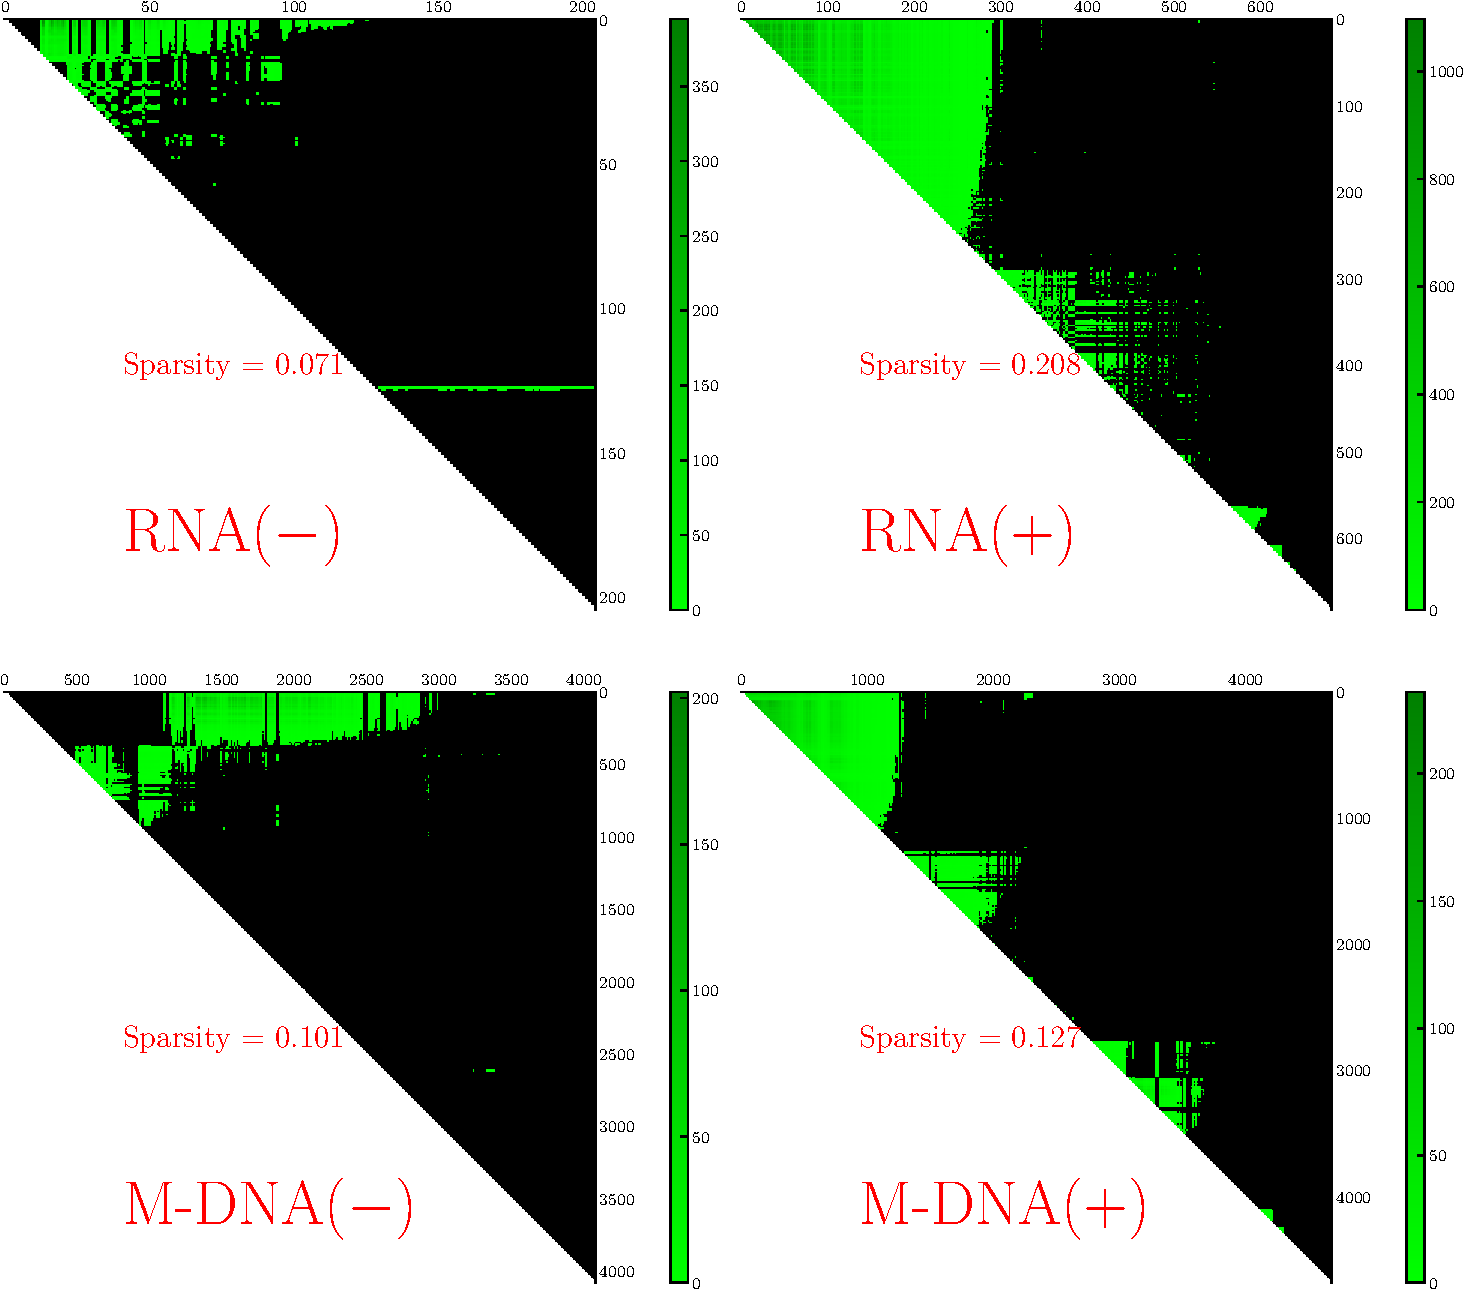
\includegraphics[scale=0.4]{clustered-matrices.pdf}
\caption{\label{fig:mat}Adjacency matrices of the projections onto RNA (top panel) and M-DNA (bottom panel) for both positive (right) and negative (left) complementary correlations. Each matrix consists in diagonal blocks representing networks connected components sorted by their size in decreasing order. Within a diagonal block, column and row index are sorted by nodes degree in decreasing order. Note that due to the symmetry of the matrices, only upper triangular parts are displayed. The sparsity of a $n\times n$ square matrix is the ratio $\frac{\sum_{i,j}A_{ij}\neq 0}{n^{2}}$.}
\end{figure}
\begin{figure}[h!]
\centering
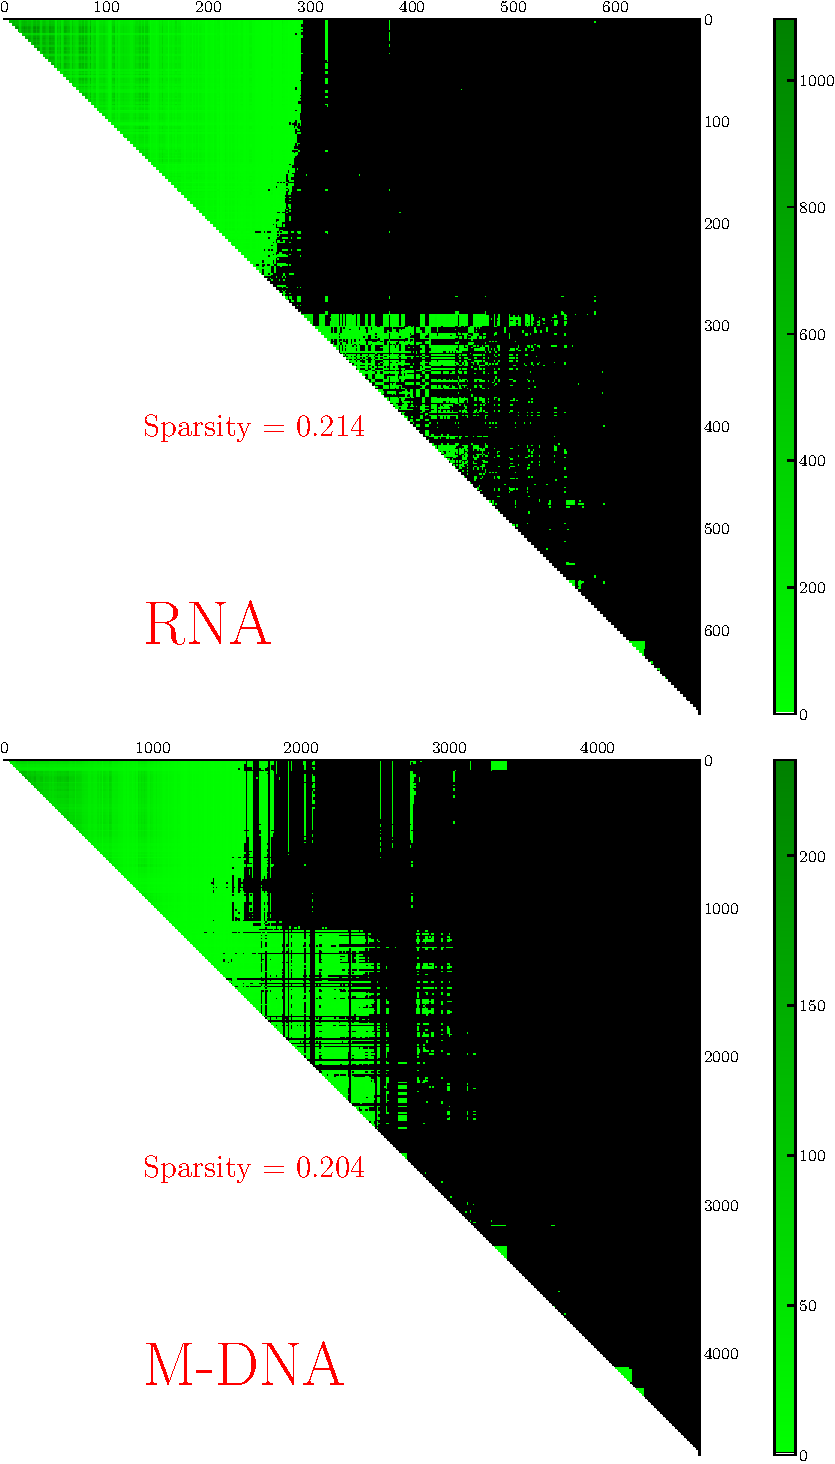
\includegraphics[scale=0.4]{clustered-matrices-mixed.pdf}
\caption{\label{fig:matmixed}Adjacency matrices of the projections onto RNA (top panel) and M-DNA (bottom panel) of mixed complementary correlations signs.}
\end{figure}


\begin{table}[h!]
\centering
\caption{\label{tab:stat}Statistics of projected networks}
\begin{tabular}{|r|c|c|c|c|c|c|c|c|c|c|c|c|}
\cline{2-13}
\multicolumn{1}{c|}{}&\multicolumn{3}{c|}{$N_{\mathrm{CC}}$}&\multicolumn{3}{c}{$N_{\mathrm{min}}$}&\multicolumn{3}{|c}{$N_{\mathrm{max}}$}&\multicolumn{3}{|c|}{$N_{\mathrm{tot}}$}\\
\cline{2-13}
\multicolumn{1}{c|}{}&$-$&$+$&$\pm$&$-$&$+$&$\pm$&$-$&$+$&$\pm$&$-$&$+$&$\pm$\\
\hline
RNAs&2&24&22&78&2&2&127&565&611&205&683&683\\
M-DNAs&2&84&83&2&2&2&4078&2763&4095&4080&4684&4687\\
\hline
\end{tabular}
\end{table}
\begin{figure}[h!]
\centering
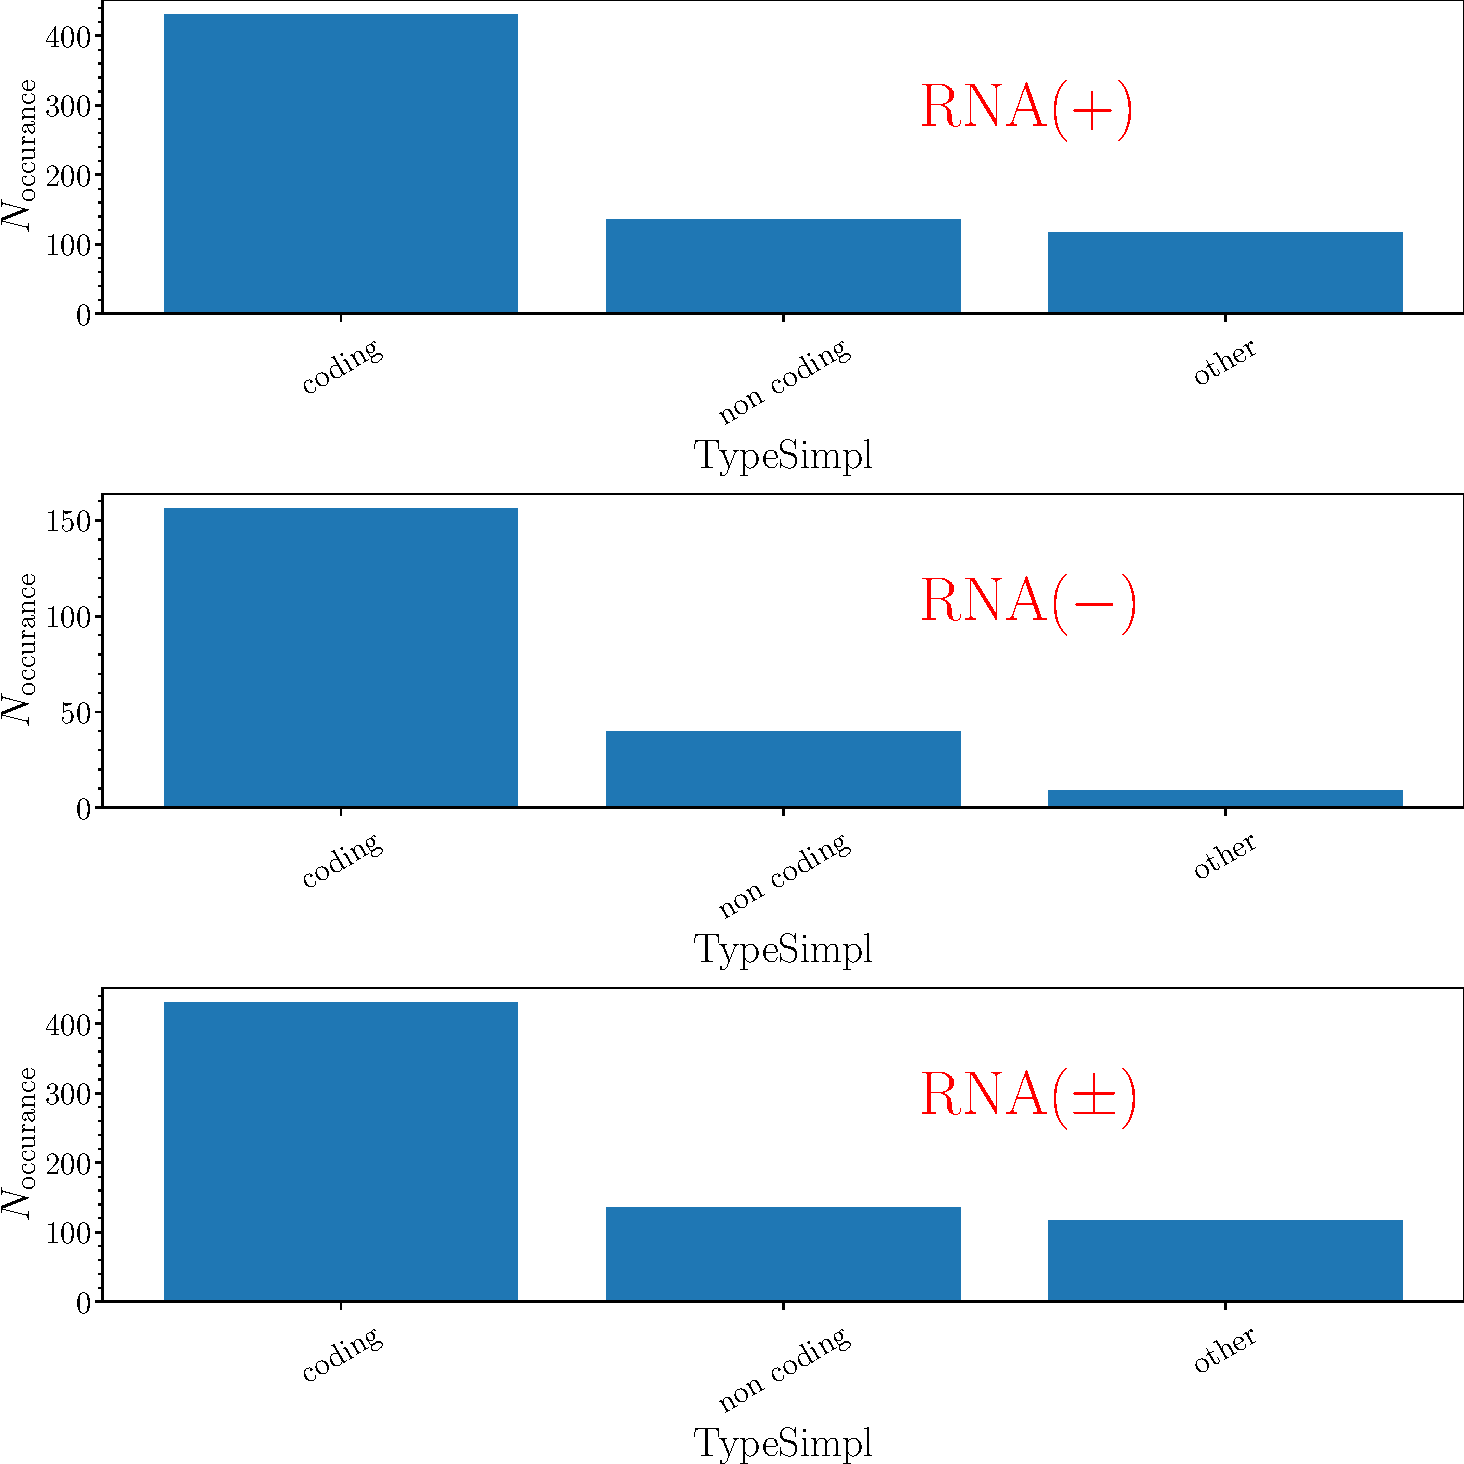
\includegraphics[scale=0.3]{dist-TypeSimpl-size.pdf}
\caption{\label{fig:TypSimpl-distr}Ditribution of RNAs present in all projections in terms of Simple Type (coding, non-coding and other). From to bottom are displayed the case of positive projections, negative projections and mixed signs projections.}
\end{figure}
\begin{figure}[h!]
\centering
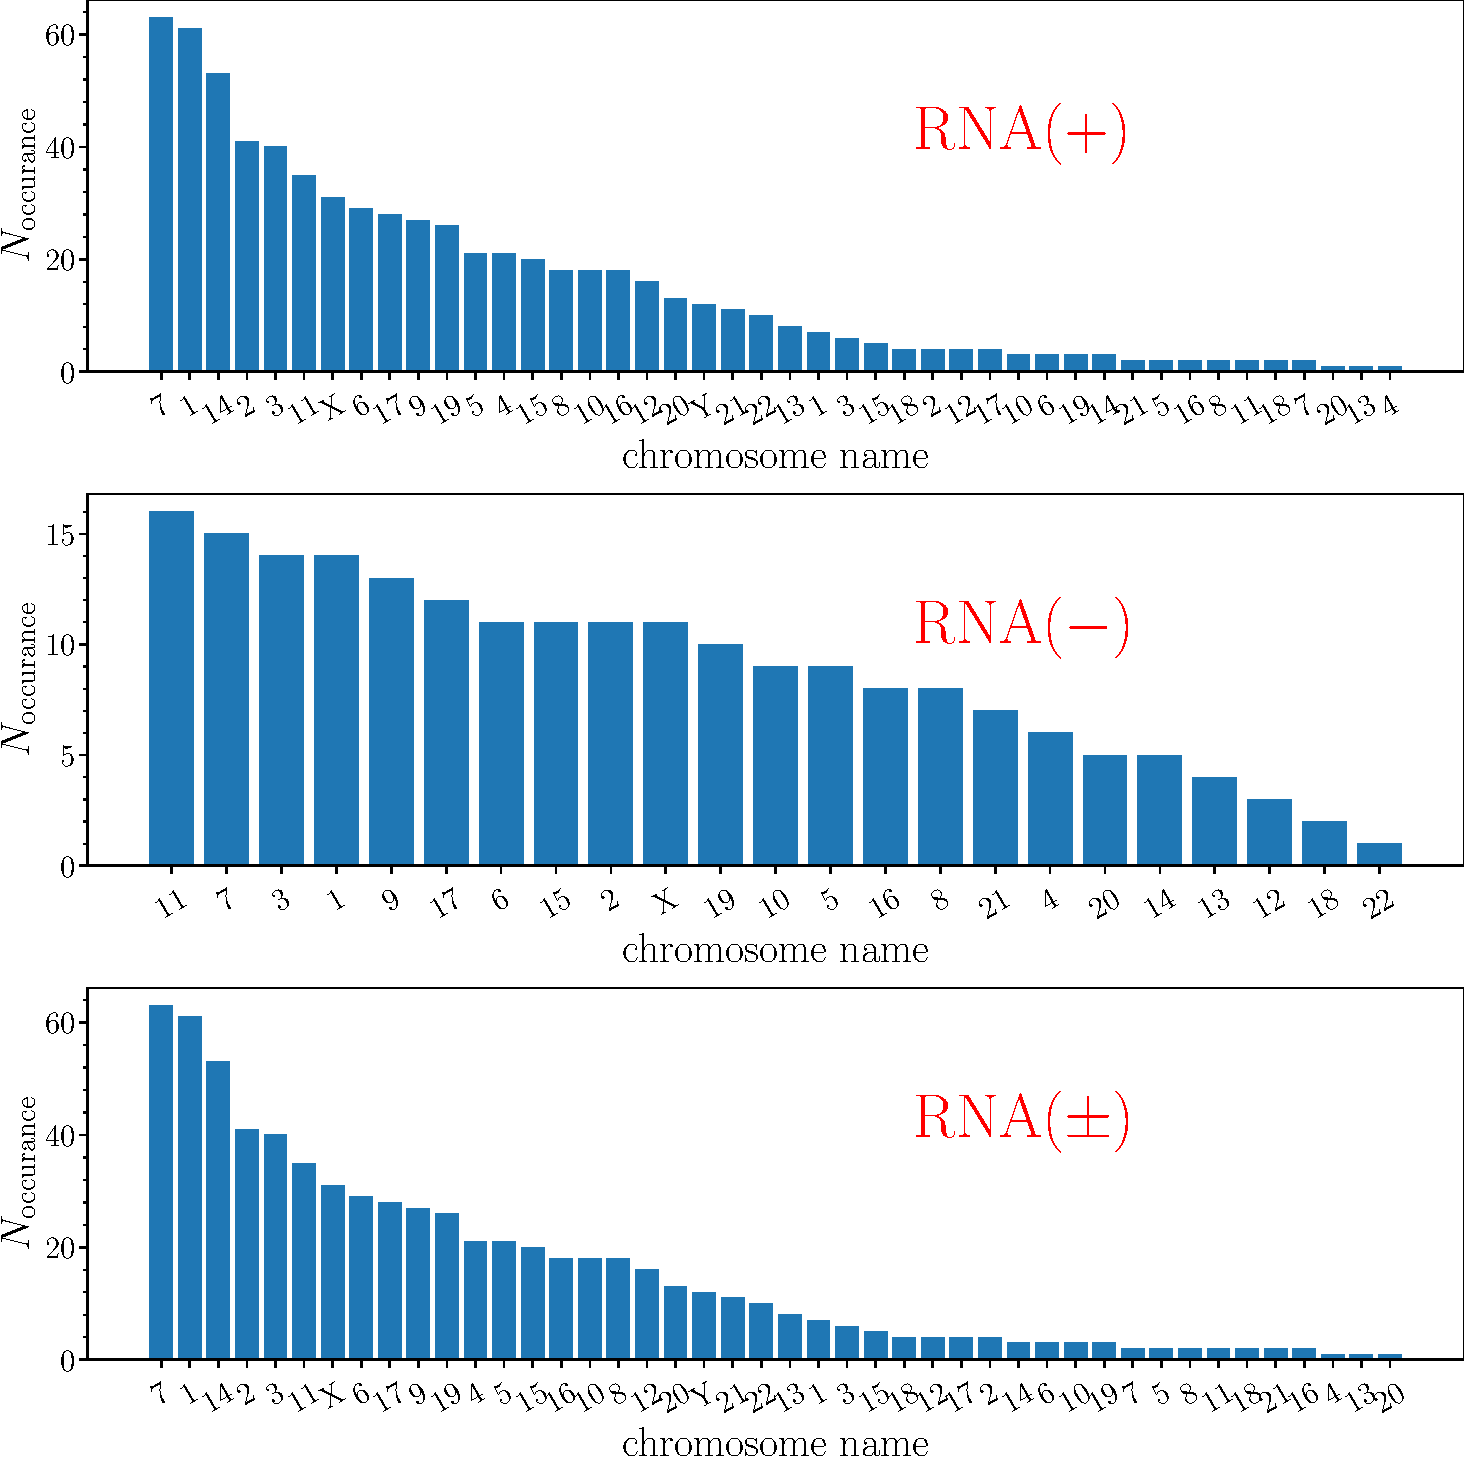
\includegraphics[scale=0.3]{dist-chromosome_name-size.pdf}
\caption{\label{fig:chromosomename-distr}Ditribution of RNAs present in all projections in terms of Chromosome Name. From to bottom are displayed the case of positive projections, negative projections and mixed signs projections.}
\end{figure}

\begin{figure}[h!]
\centering
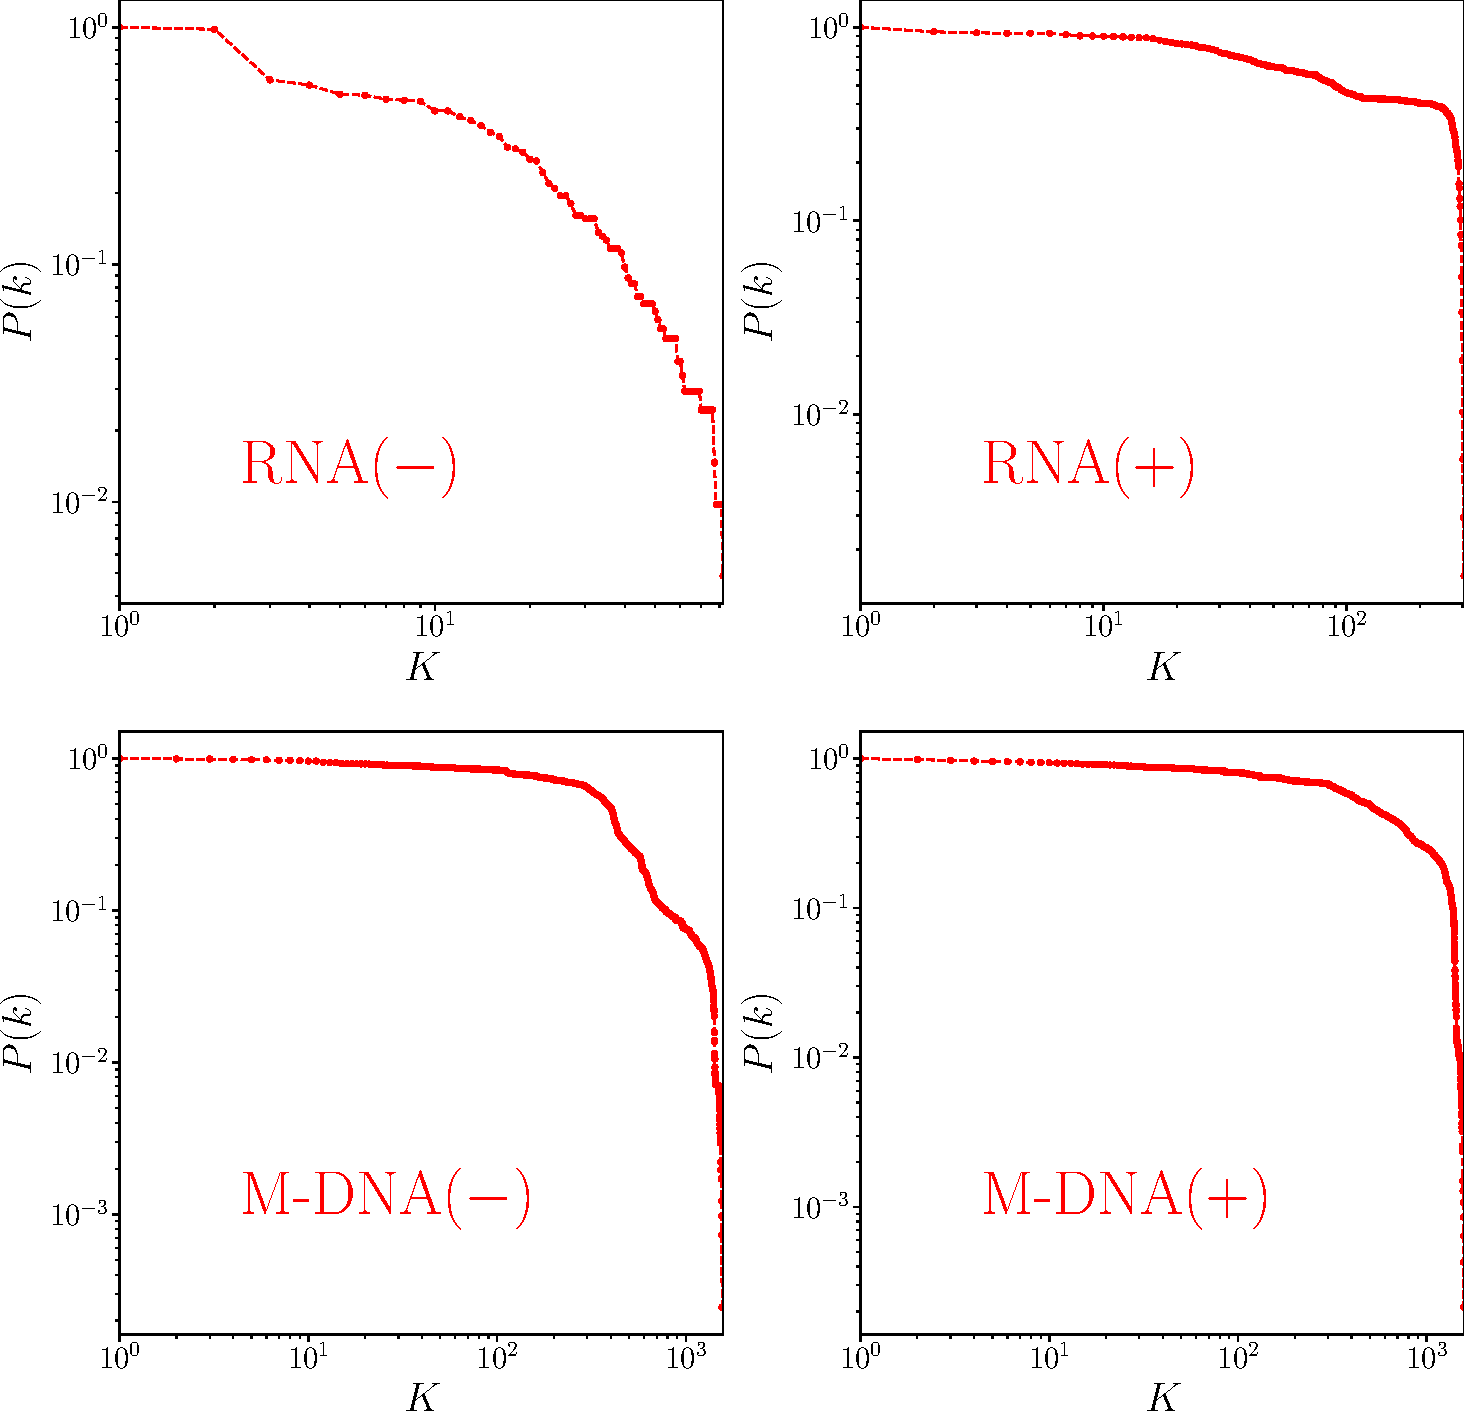
\includegraphics[scale=0.3]{degree-distr.pdf}
\caption{\label{fig:degreedistr}Cumulative degree distribution of positive and negative projected networks. $P(K)$ is the probability to find a node having at least $K$ links.}
\end{figure}
\begin{figure}[h!]
\centering
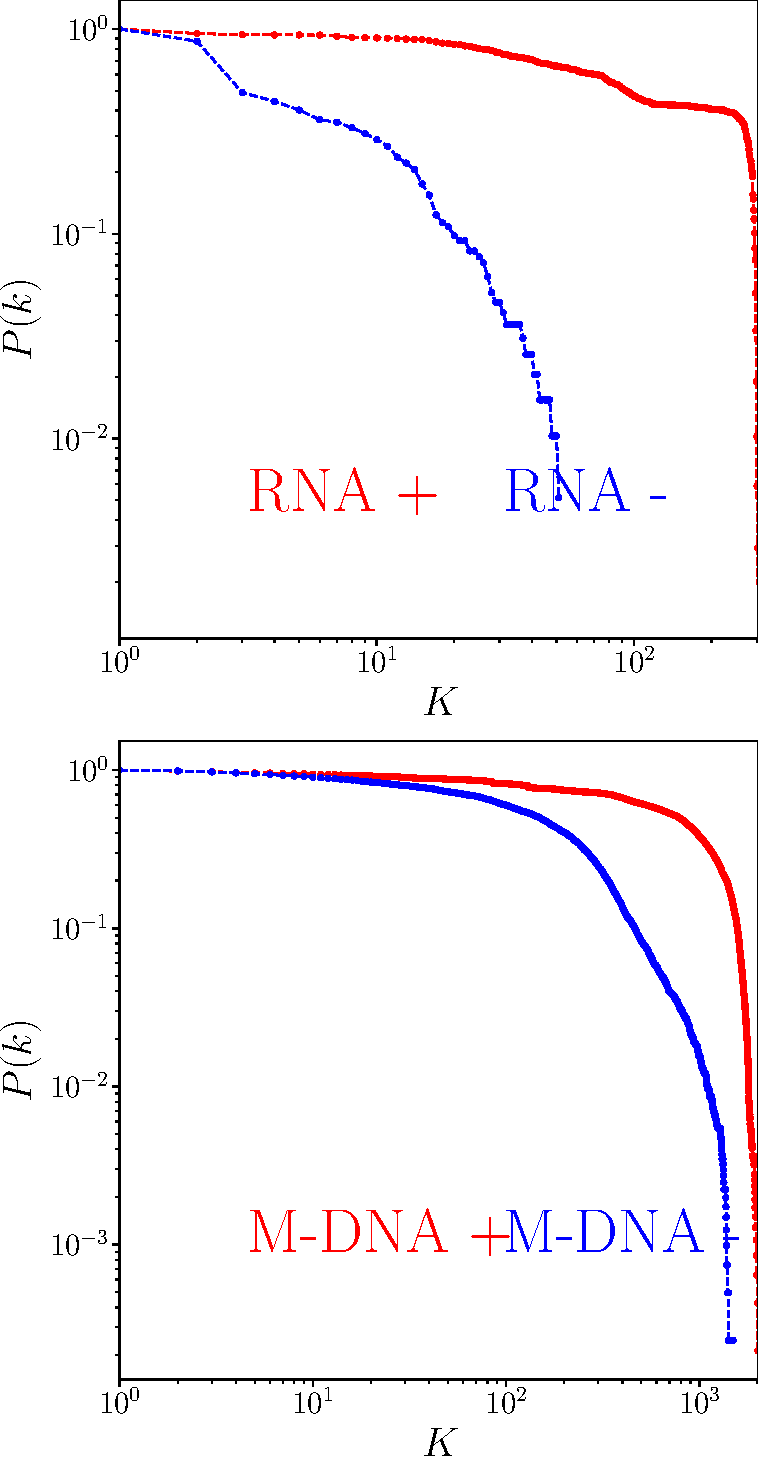
\includegraphics[scale=0.3]{degree-distr-mixed.pdf}
\caption{\label{fig:degreedistrmixed}Cumulative degree distribution of the mixed signs projected networks. $P(K)$ is the probability to find a node having at least $K$ links.}
\end{figure}

\begin{figure}[h!]
\centering
\resizebox{\columnwidth}{!}{%
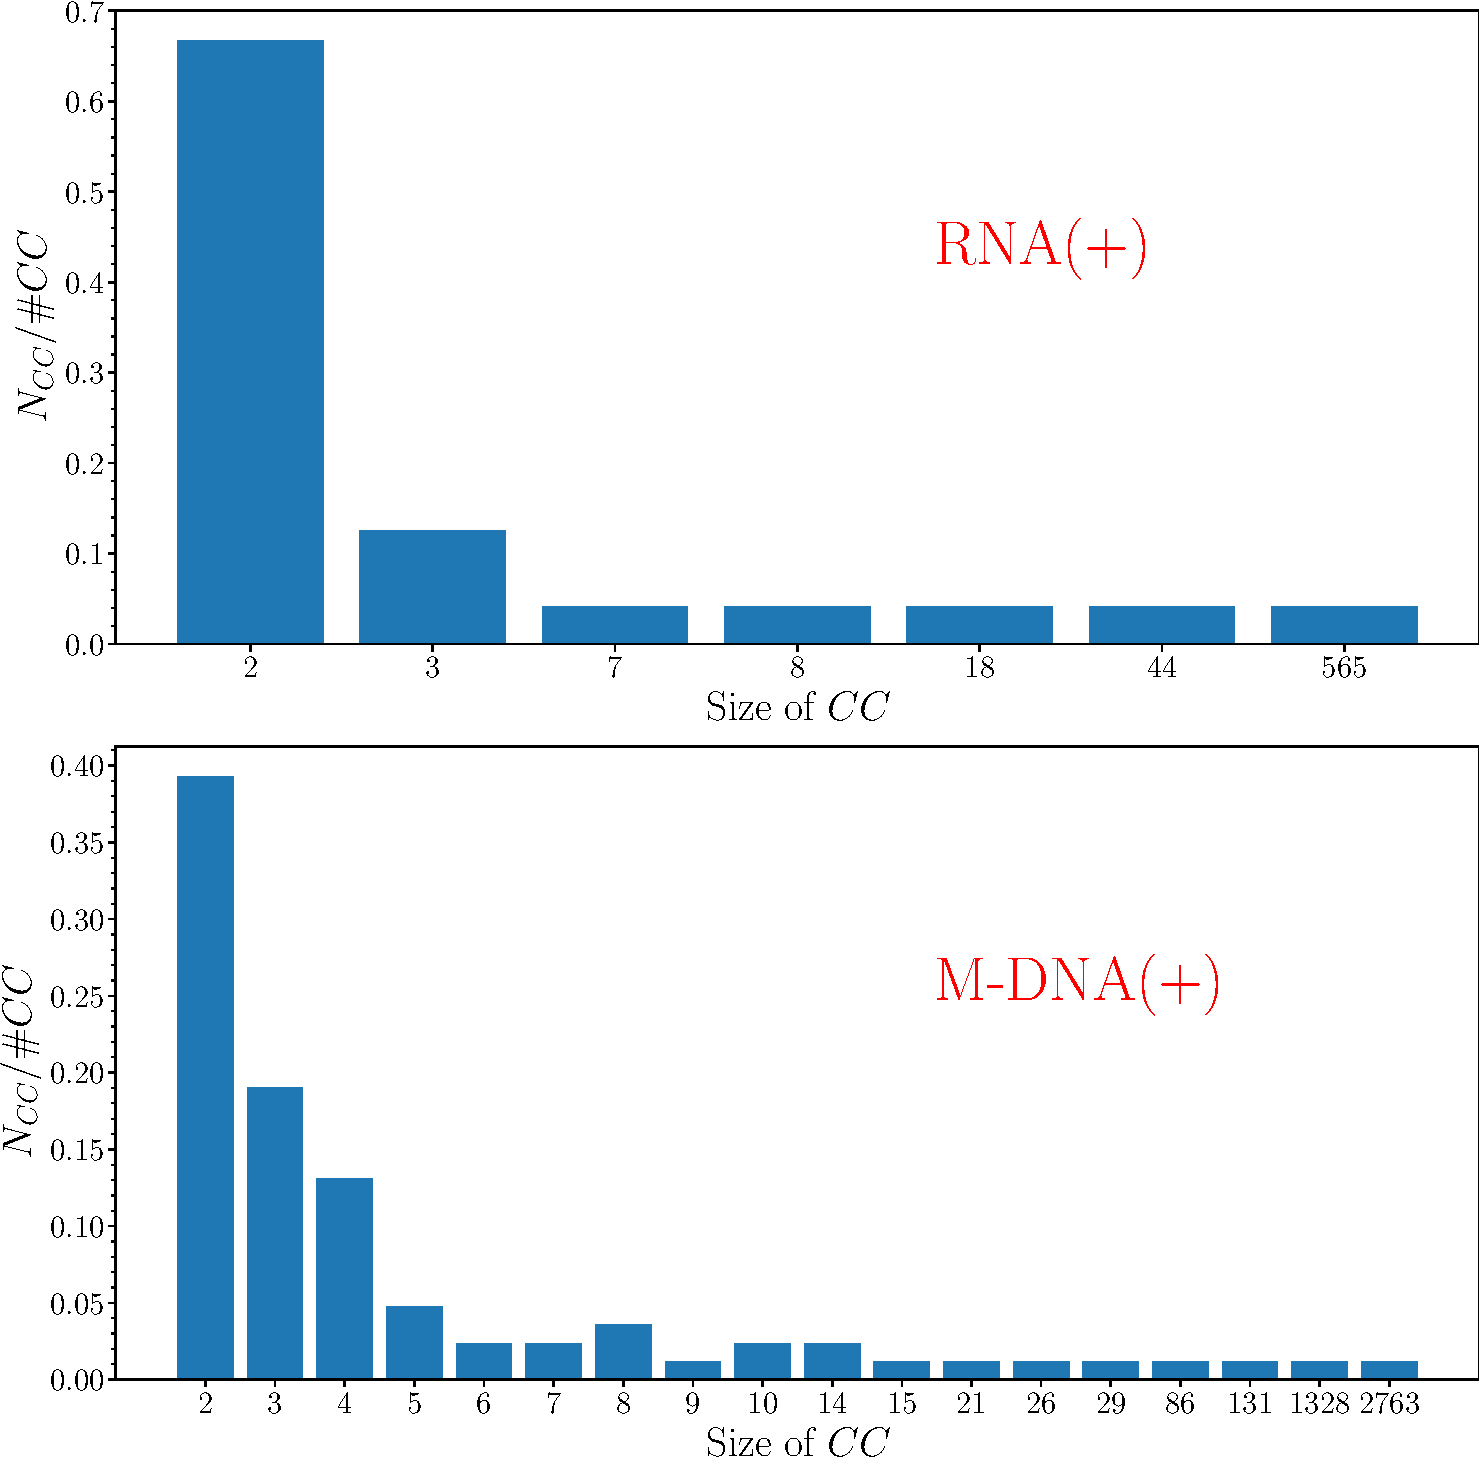
\includegraphics[scale=0.3]{dist-CC-size.pdf} 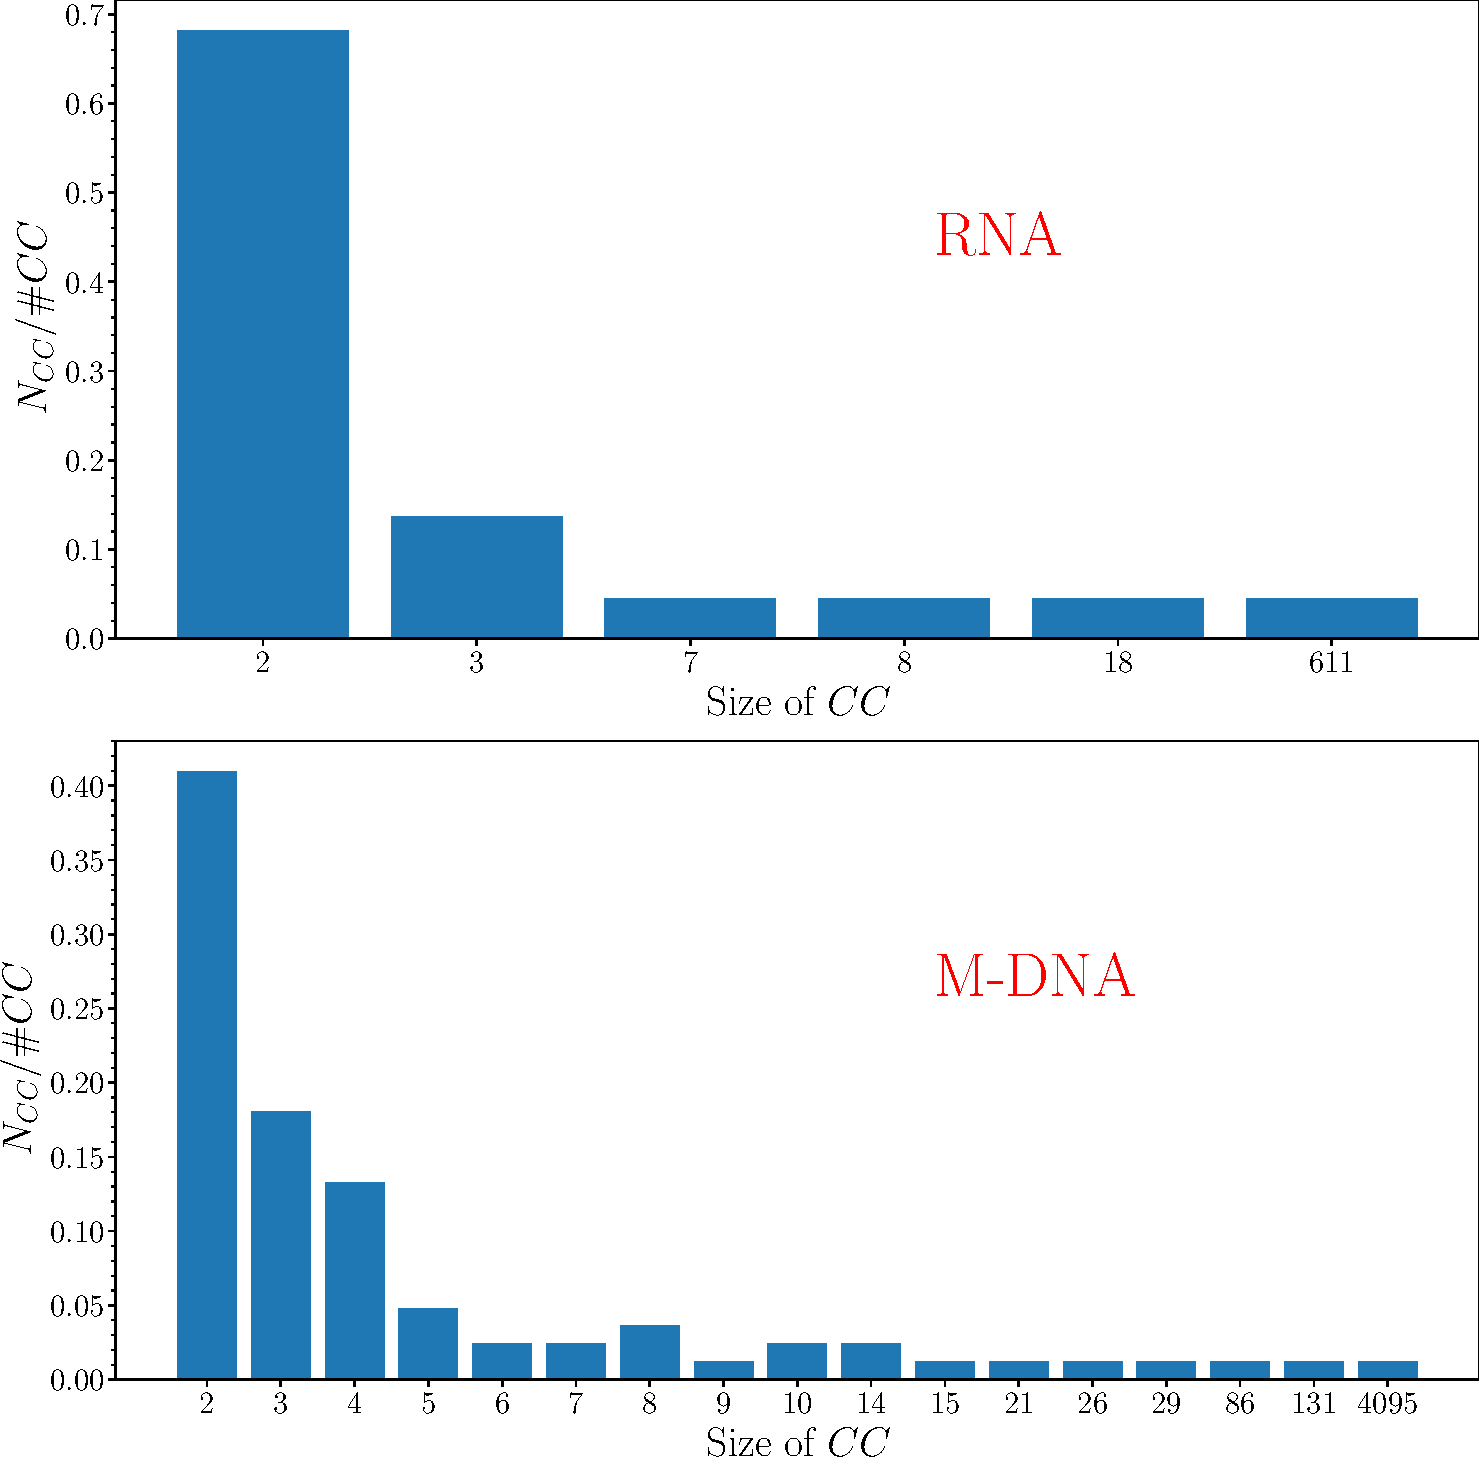
\includegraphics[scale=0.3]{dist-CC-size-mixed.pdf}
}
\caption{\label{fig:ccdistr}Distribution of the connected components size related to the positive correlation projected network (left panels) related to RNAs (top left) and M-DNAs (bottom left), and the mixed signs correlation projected network (right) for RNAs (top right) and M-DNAS (bottom right). Y-axis is the proportion of connected components.}
\end{figure}
%\begin{figure}[h!]
%\centering
%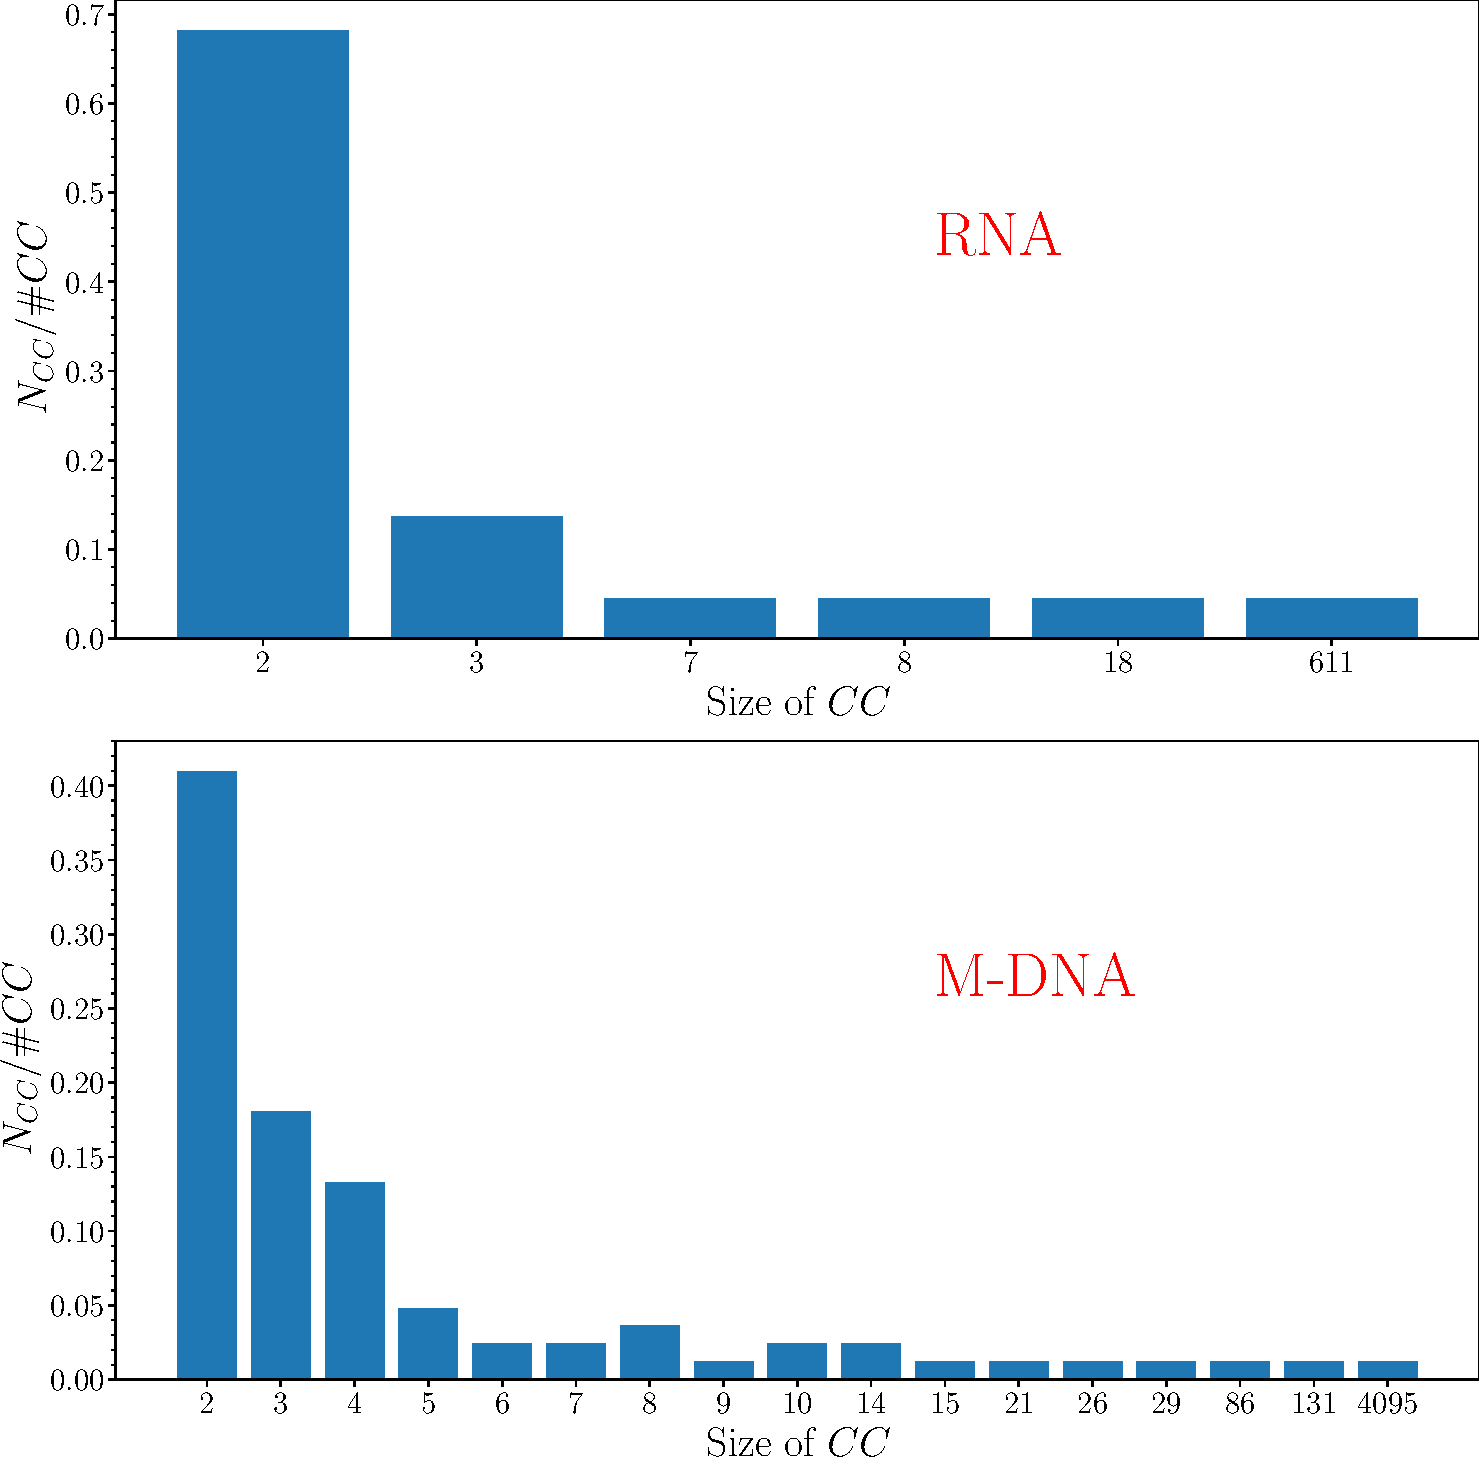
\includegraphics[scale=0.3]{dist-CC-size-mixed.pdf}
%\caption{\label{fig:ccdistrmixed}Distribution of the connected components size related to the mixed signs correlation projected network related to RNAs (top) and M-DNAs (bottom). Y-axis is the proportion of connected components.}
%\end{figure}
\clearpage
\subsection{Some very sparse networks}
The connected components of the projected networks are very dense. Indeed $\approx 90\%$ of these sub-networks are complete ($\frac{2N_{l}}{N(N-1)} = 1$). However, few of them are interestingly sparse. Fig.\ref{fig:sparsenet} presents four sparse connected components of interests.
\begin{figure}[h!]
\centering
\resizebox{0.7\columnwidth}{!}{%
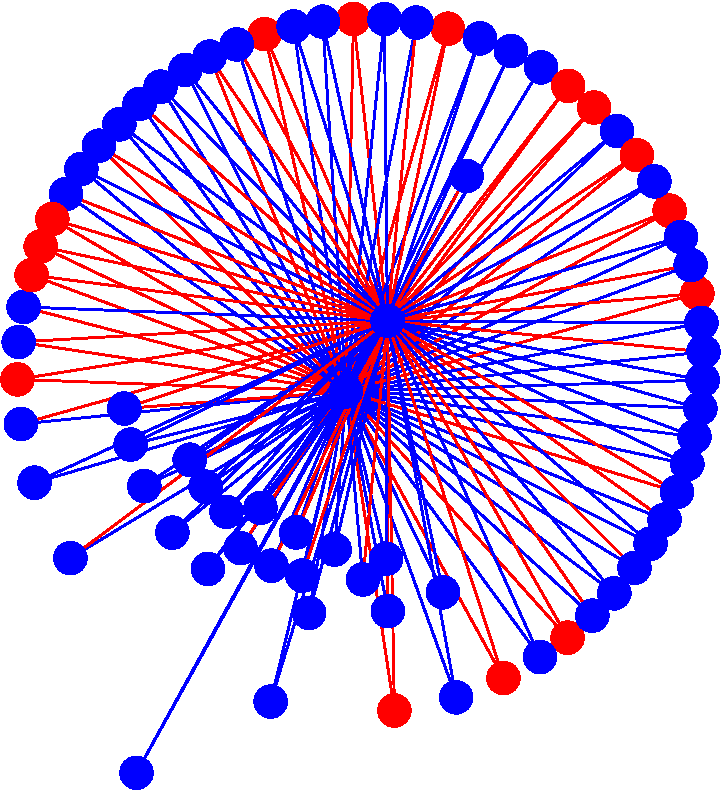
\includegraphics[width=0.4\columnwidth]{sparse-RNA-neg-CC-2.pdf} 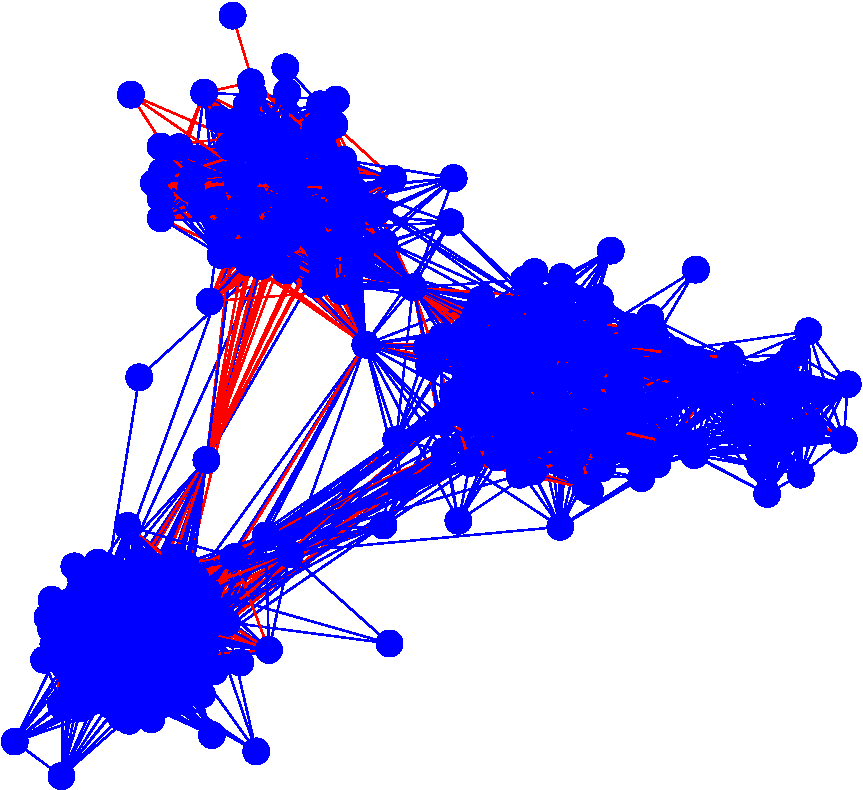
\includegraphics[width=0.4\columnwidth]{sparse-RNA-pos-CC-1.pdf}
}
\resizebox{0.7\columnwidth}{!}{%
\includegraphics[width=0.4\columnwidth]{sparse-DNA-neg-CC-1.pdf} 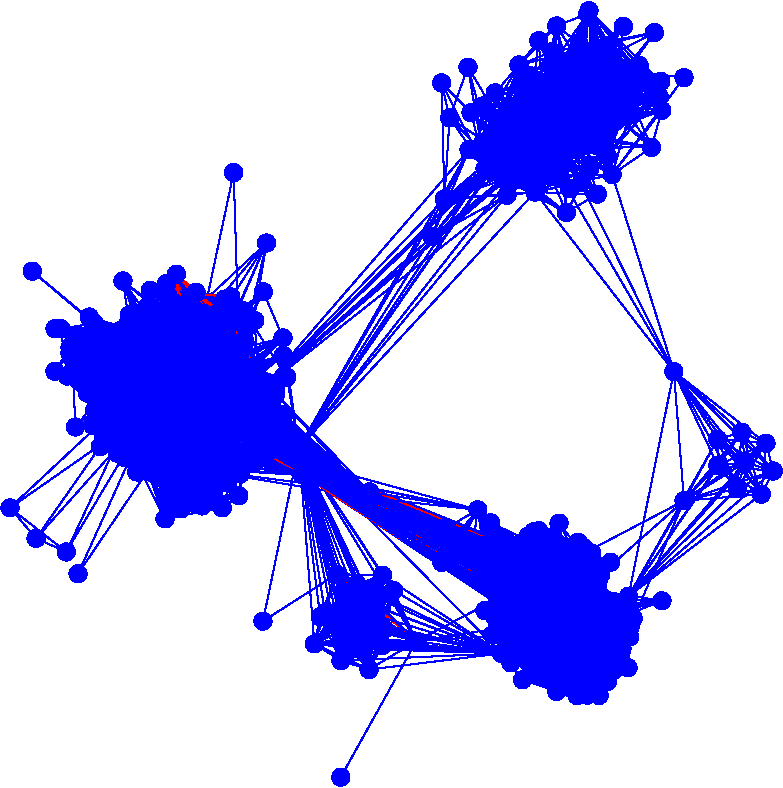
\includegraphics[width=0.4\columnwidth]{sparse-DNA-pos-CC-2.pdf}
}
\caption{\label{fig:sparsenet} Two examples of sparse networks for RNA-RNA correlations (top) and DNA-DNA correlations (bottom). Networks of negative (positive) complementary correlations are presented at the left panel (right panel). From left to right and from top to bottom, the networks' linkage density $d=\frac{2N_{l}}{N(N-1)}$ are $0.05$, $0.30$, $0.10$ and $0.24$. We show complementary correlation being present (not present) in the observed network with blue (red) links. We have $61\%$, $89\%$, $92\%$ and $98\%$ of similar links with the observed network for the top left, top right, bottom left and bottom right panel respectively. Also blue (red) nodes are nodes present (absent) in the observed correlation network. Only the top left network contains nodes being not present in the observed network ($9\%$ of the nodes).}
\end{figure}
\begin{figure}[h!]
\centering
\resizebox{0.35\columnwidth}{!}{%
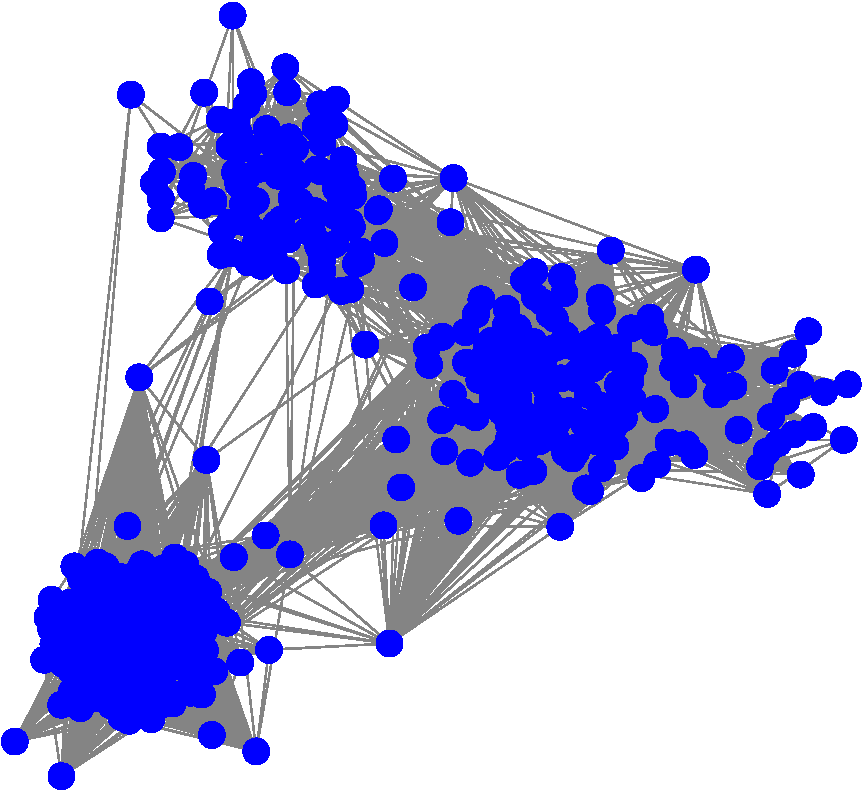
\includegraphics[width=0.2\columnwidth]{sparse-RNA-pos-CC-1-notinproj.pdf}
}
\resizebox{0.7\columnwidth}{!}{%
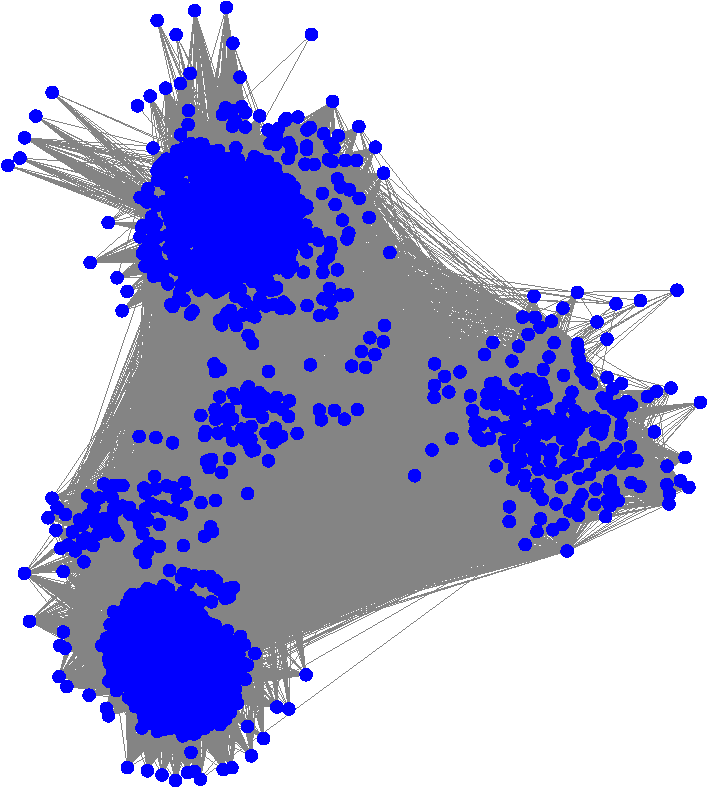
\includegraphics[width=0.4\columnwidth]{sparse-DNA-neg-CC-1-notinproj.pdf} 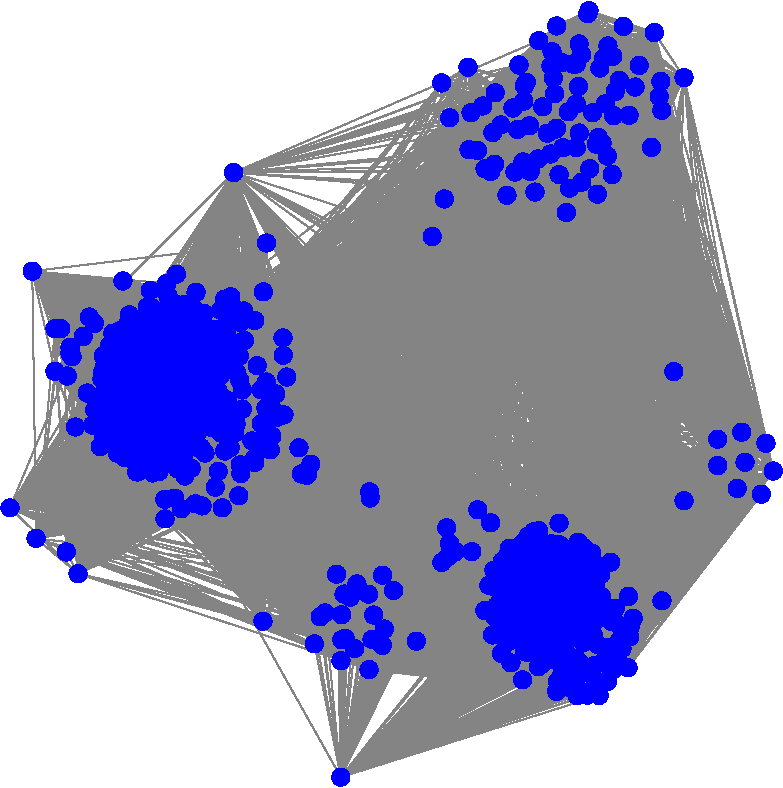
\includegraphics[width=0.4\columnwidth]{sparse-DNA-pos-CC-2-notinproj.pdf}
}
\caption{\label{fig:sparsenetnotinproj} Non-empty networks representing links between nodes of projections shown in Fig.~\ref{fig:sparsenet} that are only present in the observed networks. Top panel is related to the top left panel of Fig.~\ref{fig:sparsenet}, then the two networks in the bottom panels are related to bottom left and bottom right networks of Fig.~\ref{fig:sparsenet}.}
\end{figure}
\begin{figure}[h!]
\centering
\resizebox{0.7\columnwidth}{!}{%
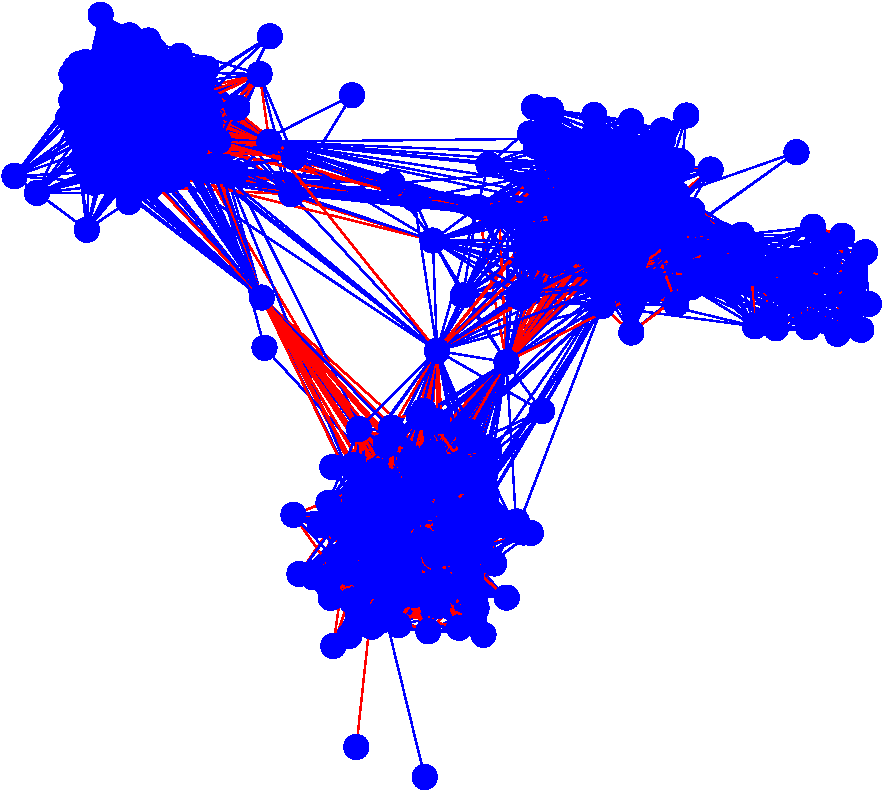
\includegraphics[width=0.4\columnwidth]{sparse-RNA-mixed-CC-1.pdf}
}
\resizebox{0.7\columnwidth}{!}{%
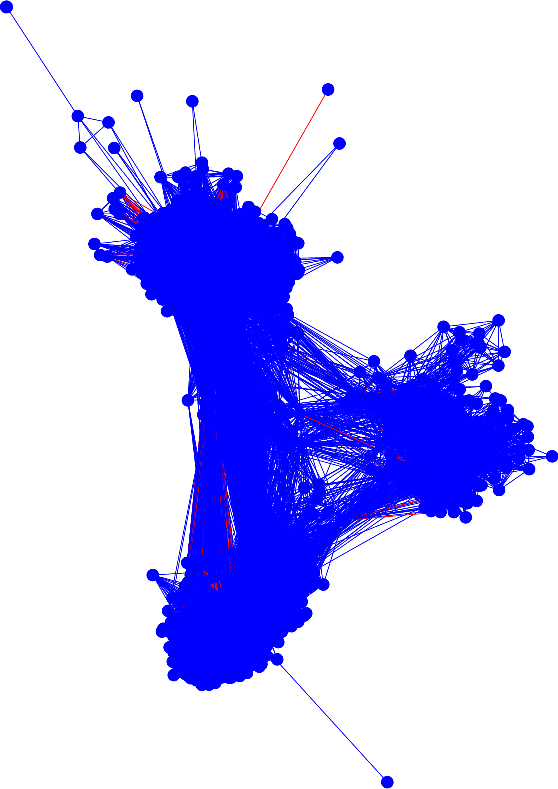
\includegraphics[width=0.4\columnwidth]{sparse-DNA-mixed-CC-1.pdf}
}
\caption{\label{fig:mixedsparsenet} Two examples of sparse networks for RNA-RNA correlations (top) and DNA-DNA correlations (bottom) obtained from mixed-sign projected networks. From top to bottom the networks' linkage density $d=\frac{2N_{l}}{N(N-1)}$ are $0.27$ and $0.26$. There are $87\%$ and $96\%$ of observed links for the left and right networks respectively.}
\end{figure}
\begin{figure}[h!]
\centering
\begin{subfigure}{0.4\textwidth}
\includegraphics[width=\textwidth]{sparse-DNA-mixed-CC-1-notinproj.pdf}
\end{subfigure}
\begin{subfigure}{0.4\textwidth}
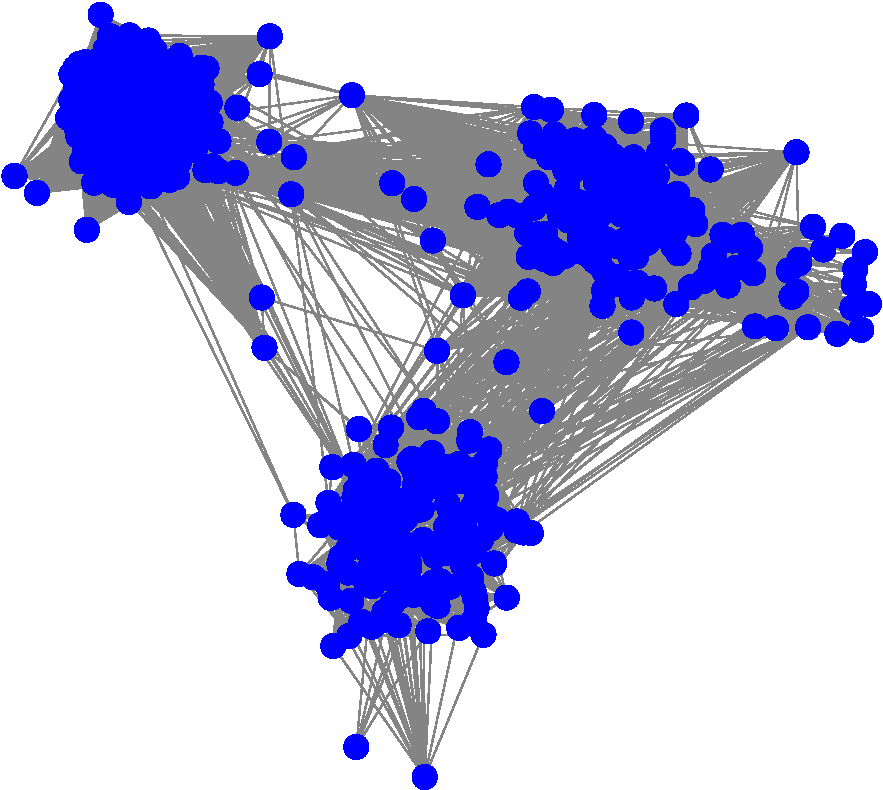
\includegraphics[width=\textwidth]{sparse-RNA-mixed-CC-1-notinproj.pdf}
\end{subfigure}
\caption{\label{fig:mixedsparsenetnotinproj} Non-empty networks representing links between nodes of projections shown in Fig.~\ref{fig:mixedsparsenet} that are only present in the observed networks. Top panel is related to the top left panel of Fig.~\ref{fig:sparsenet}, then the two networks in the bottom panels are related to bottom left and bottom right networks of Fig.~\ref{fig:sparsenet}.}
\end{figure}
\clearpage
\subsection{Some very small networks}
As we see with Fig.~\ref{fig:ccdistr}, the majority of the connected components contains few nodes $N \in [2,5]$. These small networks are very dense. We present in Fig.~\ref{fig:smallnet} two relatively dense sub-networks related to positive complementary correlations between DNAs and RNAs having few nodes.
\begin{figure}[h!]
\centering
\begin{subfigure}{0.4\textwidth}
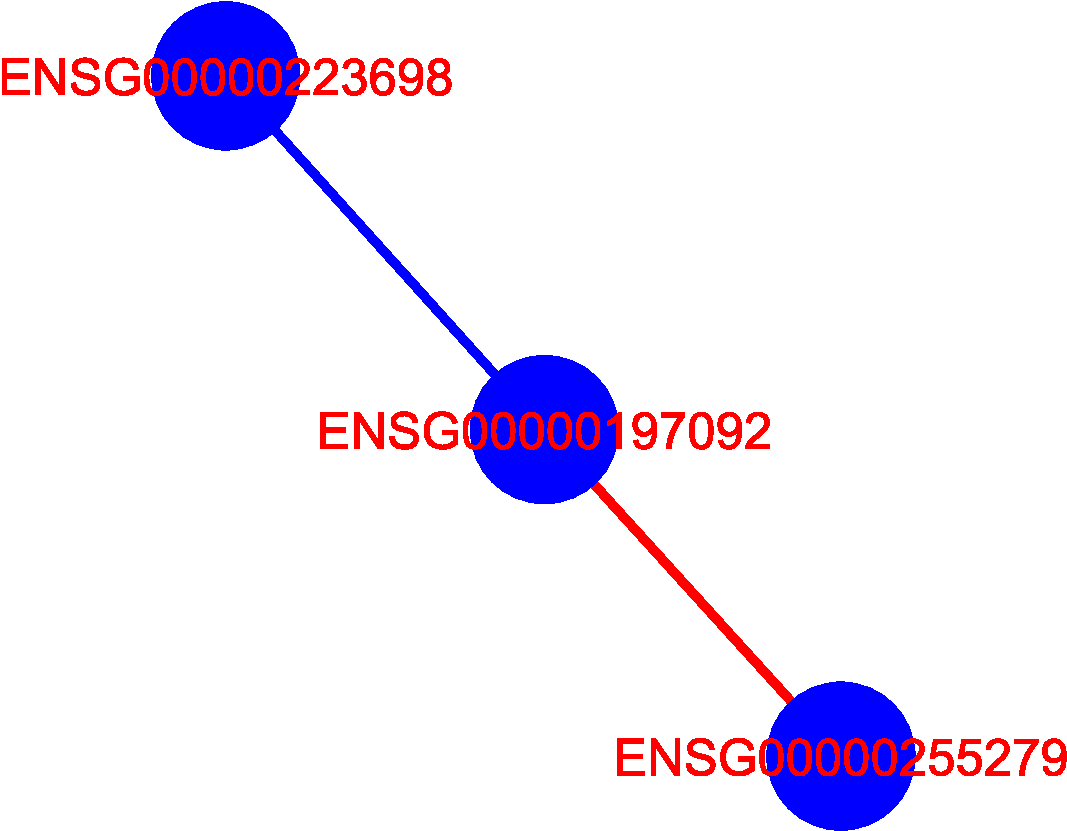
\includegraphics[width=\textwidth]{small-RNA-pos-CC-11.pdf}
\end{subfigure}
\hspace{5pt}
\begin{subfigure}{0.4\textwidth}
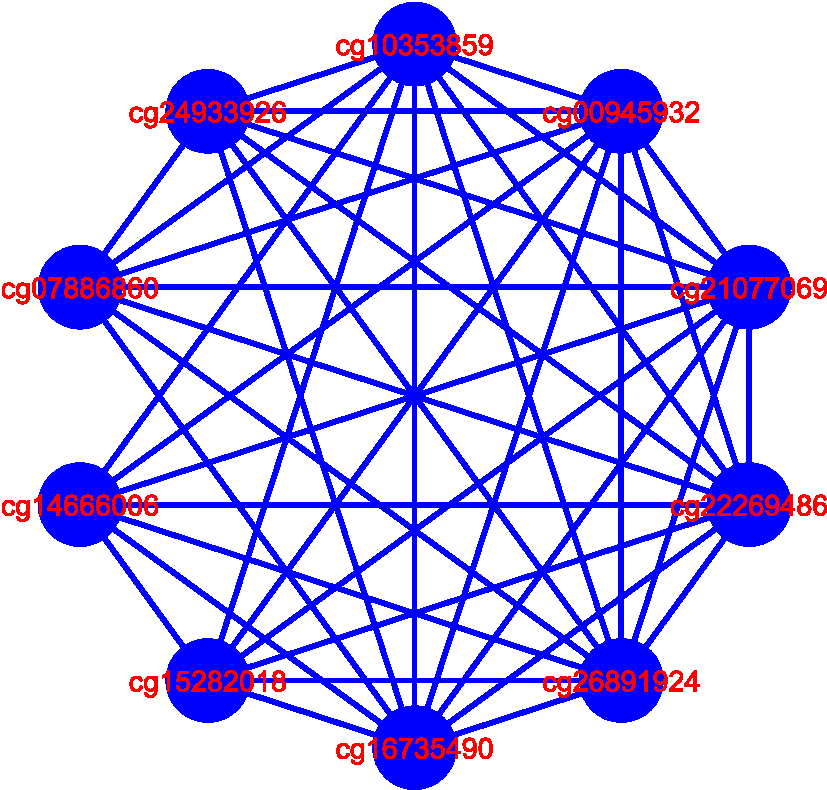
\includegraphics[width=\textwidth]{small-DNA-pos-CC-31.pdf}
\end{subfigure}
\caption{\label{fig:smallnet} Examples of small networks related to positive complementary RNA-RNA correlations (left) with $d=0.9$ and positive DNA-DNA correlations (right) with $d=0.7$.  We show complementary correlation being present (not present) in the observed network with blue (red) links. Also blue (red) nodes are nodes present (absent) in the observed correlation network.}
\end{figure}
\begin{figure}[h!]
\centering
\begin{subfigure}{0.2\textwidth}
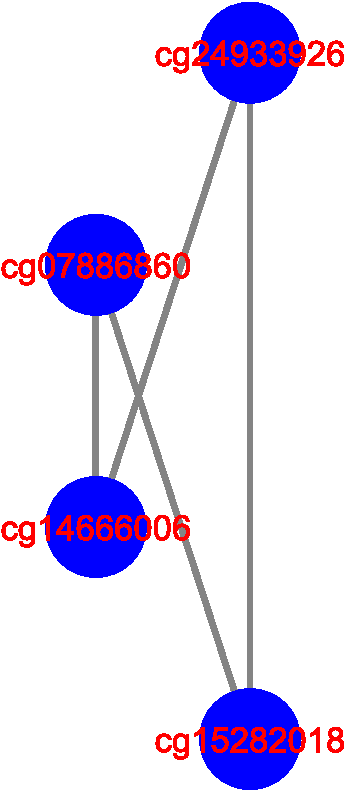
\includegraphics[width=0.5\textwidth]{small-DNA-pos-CC-31-notinproj.pdf}
\end{subfigure}
\caption{\label{fig:smallnetnotinproj} Non-empty networks representing links between nodes of projections shown in Fig.~\ref{fig:smallnet} that are only present in the observed networks. This network is related to the one from the right panel of Fig.~\ref{fig:smallnet}.}
\end{figure}
\begin{figure}[h!]
\centering
\begin{subfigure}{0.4\textwidth}
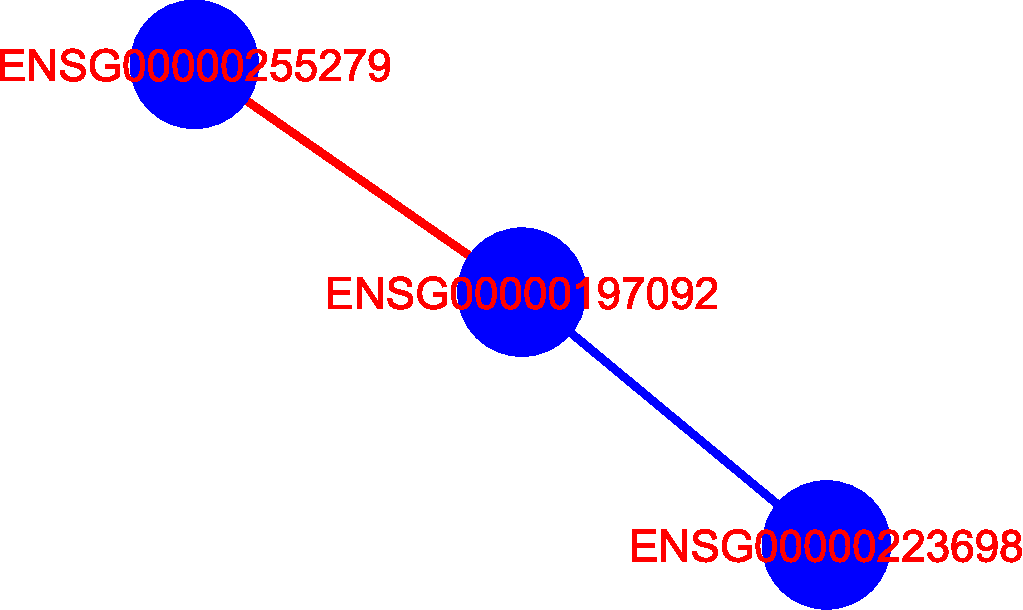
\includegraphics[width=\textwidth]{small-RNA-mixed-CC-11.pdf}
\end{subfigure}
\hspace{5pt}
\begin{subfigure}{0.4\textwidth}
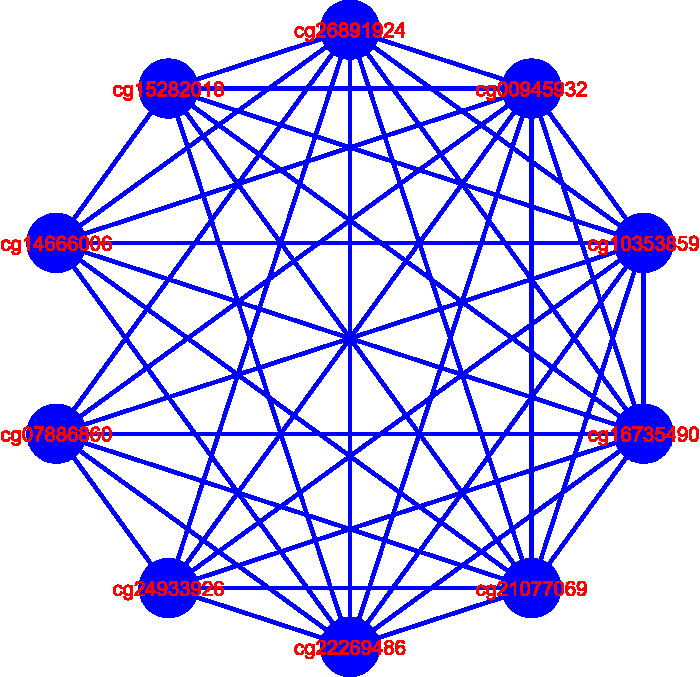
\includegraphics[width=\textwidth]{small-DNA-mixed-CC-15.pdf}
\end{subfigure}
\caption{\label{fig:mixedsmallnet} Examples of small networks obtained from mixed-sign projected networks, for RNA-RNA complementary correlations (left) and DNA-DNA ones (right). These networks have a linkage density of $67\%$ (left) and $91\%$ (right). We show complementary correlation being present (not present) in the observed network with blue (red) links. Also blue (red) nodes are nodes present (absent) in the observed correlation network.}
\end{figure}
\begin{figure}[h!]
\centering
\begin{subfigure}{0.2\textwidth}
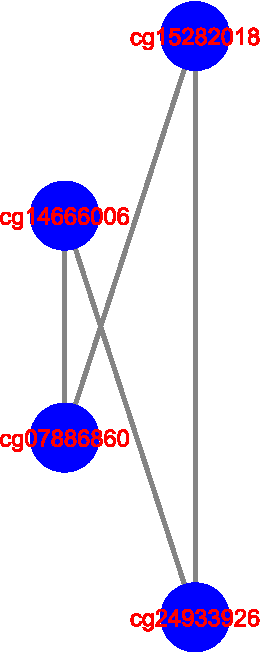
\includegraphics[width=0.5\textwidth]{small-DNA-mixed-CC-15-notinproj.pdf}
\end{subfigure}
\caption{\label{fig:mixedsmallnetnotinproj} Non-empty networks representing links between nodes of projections shown in Fig.~\ref{fig:mixedsmallnet} that are only present in the observed networks. This network is related to the one from the right panel of Fig.~\ref{fig:smallnet}.}
\end{figure}
\printbibliography


\end{document}
